% \begin{document}
\chapter{Polynomial Identity Testing and Matchings}

In this lecture we discuss polynomial identity testing and its applications:
checking whether $AB = C$ for matrices $A, B, C$ quickly, and solving the
matching problem by computing a determinant.

\section{Polynomial Identity Testing and Schwartz--Zippel Lemma}

Given polynomials $p(x)$ and $q(x)$, we want to know whether they are identical,
i.e.\ whether
\[
p(x) - q(x) = 0
\]
holds for all $x \in \R^d$.

\dfn{Monomial}{A \emph{monomial} is a product of powers of
variables with nonnegative exponents, possibly with a constant coefficient. Its
\emph{degree} is the sum of all exponents.}

\dfn{Polynomial}{A \emph{polynomial} is a sum of monomials (its
\emph{terms}). Its \emph{degree} is the largest degree of any monomial with
nonzero coefficient.}

The naive test lists all monomials of $p$ and $q$ and compares them. This is
often impractical: $\det$ has $n!$ terms. For such polynomials we only have
\emph{oracle access}: we can evaluate the polynomial at a chosen input. For
instance, setting $A_{i,j} = x_{i,j}$ to specific values, $\det(A)$ is computable
in $O(n^3)$ time via LU decomposition.

\dfn{Polynomial Identity Testing}{Given polynomials
$p$ and $q$ over a common set of variables $x$, determine whether
$p(x) - q(x) = 0$ for all values of $x$, given only oracle access: no term of
$p$ or $q$ is known, but both can be evaluated at any input $x$.}

\ex{}{ Consider a univariate polynomial of degree $n$,
\[
p(x) = a_0 x^n + a_1 x^{n-1} + \cdots + a_{n-1} x + a_n.
\]
It suffices to evaluate $p(1), p(2), \ldots, p(n+1)$. If any is nonzero, $p$ is
not identically zero. If all are zero, then $p$ has at least $n+1$ roots; by the
Fundamental Theorem of Algebra a nonzero polynomial of degree $n$ has at most $n$
real roots, so $p$ is identically zero.}

The multivariate case is harder, since multivariate polynomials can have
infinitely many roots: $x^2 - y$ has uncountably many roots (all $(x,y)$ with
$y = x^2$), so no list of roots certifies that $p \equiv 0$. Still, a nonzero
polynomial is unlikely to vanish at a random input:

\mlenma{The Schwartz--Zippel Lemma}{
Let $p(x_1, \ldots, x_n)$ be a nonzero polynomial of $n$ variables with degree
$d$. Let $S$ be a finite subset of $\R$ with at least $d$ elements. If
$x_1, \ldots, x_n$ are assigned values from $S$ independently and uniformly at
random, then
\[
\Pr[p(x_1, \ldots, x_n) = 0] \le \frac{d}{|S|}.
\]
}

So it suffices to pick $S$ and try random inputs; the probability of a false
``zero'' is small when $|S| \gg d$. No deterministic counterpart is known, and
finding one would have far-reaching consequences, with impact akin to $\mathrm{P}
= \mathrm{NP}$. We first prove a simpler instance.

\section{Matrix Identity Testing}

Given $n \times n$ matrices $A, B, C$, we want to test whether $AB = C$.
Multiplying $A$ by $B$ costs $O(n^3)$ time; randomization does better. Let
$S \subset \R$ be finite and pick $x \in \R^n$ with each coordinate drawn
independently and uniformly:
\[
x_i \sim \mathrm{Uniform}(S).
\]
Test whether $ABx = Cx$; if so, conclude $AB = C$. This costs $O(n^2)$ (three
matrix-vector products), and less for sparse matrices. How likely is a false
positive, i.e.\ $ABx = Cx$ when $AB \neq C$?

\thm{}{
If $AB \neq C$, then
\[
\Pr_{x_i \sim S}[ABx \neq Cx] \ge 1 - \frac{1}{|S|}.
\]
}

This follows from the Schwartz--Zippel Lemma, but we give a direct proof, which
also prepares the proof of the lemma.

\pf{}{
Write $AB$ and $C$ in terms of rows:
\[
AB = \begin{pmatrix} a_1 \\ \vdots \\ a_n \end{pmatrix}, \qquad
C = \begin{pmatrix} c_1 \\ \vdots \\ c_n \end{pmatrix}.
\]
Since $AB \neq C$, there is $i$ with $a_i \neq c_i$. We show
\[
\Pr[\ip{a_i}{x} \neq \ip{c_i}{x}] \ge 1 - \frac{1}{|S|}.
\]
We use the \emph{principle of deferred decision}: random choices are made only
when they become relevant. Since $a_i \neq c_i$, there is a coordinate $j$ with
$a_{i,j} \neq c_{i,j}$. Fix all $x_k$ with $k \neq j$ arbitrarily; by
independence, the randomness of $x_j$ is unaffected. The event
\begin{equation}
\sum_{k=1}^{n} a_{i,k} x_k - \sum_{k=1}^{n} c_{i,k} x_k = 0 \label{eq:ip}
\end{equation}
can be rewritten as
\begin{equation}
x_j (a_{i,j} - c_{i,j}) = -\sum_{k \neq j} (a_{i,k} - c_{i,k}) x_k. \label{eq:ip2}
\end{equation}
Since the other $x_k$ are fixed and $a_{i,j} \neq c_{i,j}$, equation
\eqref{eq:ip2} holds for at most one value of $x_j$, so
\[
\Pr_{x_j \sim S}[\ip{a_i}{x} = \ip{c_i}{x}] \le \frac{1}{|S|}.
\]
As this bound holds regardless of the values of the other $x_k$, it still holds
when they are random:
\[
\Pr_{x \sim S}[\ip{a_i}{x} = \ip{c_i}{x}] \le \frac{1}{|S|}.
\]
}

Deferred decision is a useful tool, but any analysis after fixing some variables
must hold regardless of their values (hence ``arbitrarily''). The proof of the
Schwartz--Zippel Lemma shows how \emph{not} to use it naively.

\section{Proof of Schwartz--Zippel Lemma}

\pf{Proof of the Schwartz--Zippel Lemma}{
We use strong induction on $n$.

\emph{Base case} $n = 1$: this is the univariate case of Example 2.

\emph{Inductive step.} Assume the lemma holds for all polynomials with fewer
than $n$ variables. Fix $x_1, \ldots, x_{n-1}$ arbitrarily. Then $p$ is a
univariate polynomial in $x_n$ of degree $k \le d$:
\[
p(x_n) = a_k x_n^k + a_{k-1} x_n^{k-1} + \cdots + a_1 x_n + a_0.
\]
By the univariate case,
\begin{equation}
\Pr[p(x_n) = 0] \le \frac{k}{|S|} \le \frac{d}{|S|}. \label{eq:uni}
\end{equation}
This is not enough: the probability in \eqref{eq:uni} may be affected by the
choice of $x_1, \ldots, x_{n-1}$. An adversary could choose them so that the
resulting polynomial in $x_n$ is identically $0$, giving $\Pr[p = 0] = 1$, and the
induction hypothesis implies nothing. We must argue that this adversarial
scenario is rare. To this end we use polynomial long division: for $p(x)$ of
degree $d$ and divisor $d(x)$ of degree $k \le d$, we can write
\[
p(x) = d(x) q(x) + r(x),
\]
where the quotient $q$ has degree at most $d - k$ and the remainder $r$ has
degree at most $k - 1$.

Let $k$ be the largest exponent of $x_n$ over all monomials of $p$. Dividing by
$x_n^k$,
\[
p(x_1, \ldots, x_n) = x_n^k\, q(x_1, \ldots, x_{n-1}) + r(x_1, \ldots, x_n),
\]
where $q$ is a nonzero polynomial in $x_1, \ldots, x_{n-1}$ of degree $d - k$ and
the degree of $x_n$ in $r$ is at most $k - 1$.

We again use deferred decision: first assign $x_1, \ldots, x_{n-1}$ uniformly at
random from $S$, saving the randomness of $x_n$. By the induction hypothesis,
\begin{equation}
\Pr_{x_1, \ldots, x_{n-1} \sim S}[q(x_1, \ldots, x_{n-1}) = 0] \le \frac{d-k}{|S|}. \label{eq:q}
\end{equation}
If $q \neq 0$, then $p$ is a univariate polynomial in $x_n$ whose coefficient of
$x_n^k$ is nonzero, hence $p$ is not identically $0$ and has degree $k$. So for
random $x_n \in S$,
\begin{equation}
\Pr_{x_n \sim S}[p = 0 \mid q \neq 0] \le \frac{k}{|S|}. \label{eq:pq}
\end{equation}
Combining \eqref{eq:q} and \eqref{eq:pq},
\begin{align*}
\Pr[p = 0] &= \Pr[p = 0 \mid q = 0] \Pr[q = 0] + \Pr[p = 0 \mid q \neq 0] \Pr[q \neq 0] \\
           &\le \Pr[q = 0] + \Pr[p = 0 \mid q \neq 0] \\
           &\le \frac{d-k}{|S|} + \frac{k}{|S|} = \frac{d}{|S|}.
\end{align*}
}

\section{Bipartite Graph Matching}

Polynomial identity testing can decide whether a bipartite graph
$G = (X, Y, E)$ has a perfect matching.

A deterministic algorithm finds a perfect matching in time
$O(|E|\sqrt{|X| + |Y|})$. We build a randomized one. Assume $|X| = |Y| = n$ (else
no perfect matching exists) and define the matrix
\[
A_{ij} =
\begin{cases}
x_{ij} & \text{if } x_i \text{ and } y_j \text{ are joined by an edge,} \\
0 & \text{otherwise.}
\end{cases}
\]

\ex{}{ Consider the bipartite graph below with edges
$u_1v_1$, $u_2v_2$, $u_2v_3$, $u_3v_2$, $u_3v_3$ and matrix
\[
A = \begin{pmatrix}
x_{u_1 v_1} & 0 & 0 \\
0 & x_{u_2 v_2} & x_{u_2 v_3} \\
0 & x_{u_3 v_2} & x_{u_3 v_3}
\end{pmatrix}.
\]
\begin{center}
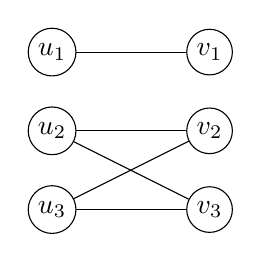
\begin{tikzpicture}[every node/.style={circle, draw, inner sep=2pt}]
  \node (u1) at (0,2) {$u_1$};
  \node (u2) at (0,1) {$u_2$};
  \node (u3) at (0,0) {$u_3$};
  \node (v1) at (2,2) {$v_1$};
  \node (v2) at (2,1) {$v_2$};
  \node (v3) at (2,0) {$v_3$};
  \draw (u1)--(v1);
  \draw (u2)--(v2);
  \draw (u2)--(v3);
  \draw (u3)--(v2);
  \draw (u3)--(v3);
\end{tikzpicture}
\end{center}
Then
\[
\det(A) = x_{u_1 v_1} x_{u_2 v_2} x_{u_3 v_3} - x_{u_1 v_1} x_{u_2 v_3} x_{u_3 v_2},
\]
where the two monomials correspond to the two perfect matchings.}

\thm{}{
$G$ has a perfect matching if and only if $\det(A)$ is not identically zero.
}

\pf{}{
$(\Rightarrow)$ Suppose $G$ has a perfect matching, i.e.\ a bijection $f$ mapping
each $x_i \in X$ to a unique $y_j \in Y$ (unique since no two matched edges share
a vertex; onto since the matching is perfect). Viewing $f$ as a permutation of
$[n]$,
\[
\prod_{i=1}^{n} A_{i,f(i)} = \prod_{i=1}^{n} x_{i,f(i)}
\]
is a nonzero monomial of $\det(A) = \sum_{\sigma} \mathrm{sgn}(\sigma)
\prod_{i=1}^n A_{i,\sigma(i)}$, arising at $\sigma = f$ with nonzero coefficient.
It differs from all other monomials of $\det(A)$, so there is no cancellation and
$\det(A)$ is not the zero polynomial.

$(\Leftarrow)$ Suppose $\det(A)$ is not identically zero, i.e.\ it is nonzero for
some values of the $x_{ij}$. Then for at least one permutation
$\sigma : [n] \to [n]$, all terms $A_{i,\sigma(i)}$, $1 \le i \le n$, are
variables $x_{i,\sigma(i)}$ rather than zeros. Hence each $x_i \in X$ is matched
to $y_{\sigma(i)} \in Y$, and since $\sigma$ is a bijection, this matching is
perfect.
}

This gives a simple, efficient test. By the Schwartz--Zippel Lemma it suffices to
assign each $x_{i,j}$ a value from a set $S$ with $|S| \ge n^2$: if $G$ has a
perfect matching, then $\det(A) \neq 0$ with probability at least $1 - 1/n$.

The test does not \emph{find} the perfect matching. To do so, choose a large set
$S$ with $|S| \gg n$ and set $x_{ij} = 2^{w_{ij}}$, where each $w_{ij}$ is chosen
independently and uniformly at random from $S$. With high probability there is a
unique minimum-weight perfect matching (see exercises), so
\[
\det(A) = 2^{w(M)} \left(\pm 1 + [\text{even number}]\right),
\]
where $w(M)$ is the total weight of the edges of the minimum-weight perfect
matching $M$. Then $w(M)$ is determined by $\det(A)$: it is the largest exponent
of $2$ dividing $\det(A)$. For every edge $(x_i, y_j)$, delete the edge and test
whether the minimum perfect matching weight drops to $w(M) - w_{i,j}$ (as read off
from the new determinant); if so, $(x_i, y_j) \in M$, and otherwise it is not.
This algorithm can be implemented in parallel in $O(\mathrm{polylog}(n))$ time
with polynomially many processors.

\section{Remarks on General Graph Matching}

The idea generalizes to perfect matchings in general graphs, though the proof is
considerably harder. Construct the skew-symmetric matrix (the \emph{Tutte
matrix})
\[
A_{ij} =
\begin{cases}
x_{ij} & \text{if } v_i \text{ and } v_j \text{ are joined by an edge, } i < j, \\
-x_{ij} & \text{if } v_i \text{ and } v_j \text{ are joined by an edge, } i \ge j, \\
0 & \text{otherwise.}
\end{cases}
\]

\thm{}{
$G$ has a perfect matching if and only if $\det(A)$ is not identically zero.
}

We omit the proof. To avoid the $O(n^3)$ cost of computing the determinant, note
there is a parallel algorithm computing it with $\mathrm{poly}(n)$ processors in
$O(\log^2 n)$ time.
% \end{document}
